% ---------------------------------------------------------------------------- %
%  Description:                                                                %
%                                                                              %
%  Author(s): 
%  Date: 
% ---------------------------------------------------------------------------- %
%\documentclass[conference]{IEEEtran}
\documentclass[a4paper,11pt]{article}

\usepackage{cite}

\usepackage[dvips]{graphicx}
% declare the path(s) where your graphic files are
\graphicspath{{./Pictures/}}
\DeclareGraphicsExtensions{.eps, .png}

% *** MATH PACKAGES ***
%
\usepackage[cmex10]{amsmath}
% A popular package from the American Mathematical Society that provides
% many useful and powerful commands for dealing with mathematics. If using
% it, be sure to load this package with the cmex10 option to ensure that
% only type 1 fonts will utilized at all point sizes. Without this option,
% it is possible that some math symbols, particularly those within
% footnotes, will be rendered in bitmap form which will result in a
% document that can not be IEEE Xplore compliant!
%
% Also, note that the amsmath package sets \interdisplaylinepenalty to 10000
% thus preventing page breaks from occurring within multiline equations. Use:
%\interdisplaylinepenalty=2500
% after loading amsmath to restore such page breaks as IEEEtran.cls normally
% does. amsmath.sty is already installed on most LaTeX systems. The latest
% version and documentation can be obtained at:
% http://www.ctan.org/tex-archive/macros/latex/required/amslatex/math/
\usepackage{amssymb,amsthm}

\usepackage{algorithm}
\usepackage{algpseudocode}
\usepackage{pstricks,pst-node}
\usepackage{pstricks-add}
\usepackage{psfrag}
%\usepackage[sort]{natbib}
\usepackage{times}
% *** SUBFIGURE PACKAGES ***
\usepackage[tight,footnotesize]{subfigure}
% subfigure.sty was written by Steven Douglas Cochran. This package makes it
% easy to put subfigures in your figures. e.g., "Figure 1a and 1b". For IEEE
% work, it is a good idea to load it with the tight package option to reduce
% the amount of white space around the subfigures. subfigure.sty is already
% installed on most LaTeX systems. The latest version and documentation can
% be obtained at:
% http://www.ctan.org/tex-archive/obsolete/macros/latex/contrib/subfigure/
% subfigure.sty has been superceeded by subfig.sty.
%\usepackage{rressched}

\newtheorem{theorem}{Theorem}
\newtheorem{lemma}{Lemma}
\newtheorem{definition}{Definition}
\newtheorem{assumption}{Assumption}
% *** Do not adjust lengths that control margins, column widths, etc. ***
% *** Do not use packages that alter fonts (such as pslatex).         ***
% There should be no need to do such things with IEEEtran.cls V1.6 and later.
% (Unless specifically asked to do so by the journal or conference you plan
% to submit to, of course. )


% correct bad hyphenation here
%\hyphenation{op-tical net-works semi-conduc-tor}


\begin{document}

%% Commands
\newcommand{\floor}[1]{\left\lfloor{#1}\right\rfloor}
\newcommand{\setof}[1]{\left\{{#1}\right\}}
\newcommand{\set}[2]{\left\{{#1}\mid{#2}\right\}}
\newcommand{\ceiling}[1]{\left\lceil{#1}\right\rceil}

\newcommand{\algorithmicinput}{\textbf{Input:}}
\newcommand{\INPUT}{\item[\algorithmicinput]}
\newcommand{\algorithmicoutput}{\textbf{Output:}}
\newcommand{\OUTPUT}{\item[\algorithmicoutput]}
\newcommand{\todo}[1]{\textcolor{blue}{TODO: #1}}

%%
%% PEPPE: Possible titles:

% \title{Reactive Reconfiguration of Bandwidth Allocation in Wireless
%   Sensor Networks}

\title{Neural Networks PhD Course Activity Report}

\author{ Mario Bambagini, Francesco Prosperi \\
\{name.surname@sssup.it\}\\
Scuola Superiore Sant'Anna, Pisa 
}

% conference papers do not typically use \thanks and this command
% is locked out in conference mode. If really needed, such as for
% the acknowledgment of grants, issue a \IEEEoverridecommandlockouts
% after \documentclass

% for over three affiliations, or if they all won't fit within the width
% of the page, use this alternative format:
%
%\author{\IEEEauthorblockN{Michael Shell\IEEEauthorrefmark{1},
%Homer Simpson\IEEEauthorrefmark{2},
%James Kirk\IEEEauthorrefmark{3},
%Montgomery Scott\IEEEauthorrefmark{3} and
%Eldon Tyrell\IEEEauthorrefmark{4}}
%\IEEEauthorblockA{\IEEEauthorrefmark{1}School of Electrical and Computer Engineering\\
%Georgia Institute of Technology,
%Atlanta, Georgia 30332--0250\\ Email: see http://www.michaelshell.org/contact.html}
%\IEEEauthorblockA{\IEEEauthorrefmark{2}Twentieth Century Fox, Springfield, USA\\
%Email: homer@thesimpsons.com}
%\IEEEauthorblockA{\IEEEauthorrefmark{3}Starfleet Academy, San Francisco, California 96678-2391\\
%Telephone: (800) 555--1212, Fax: (888) 555--1212}
%\IEEEauthorblockA{\IEEEauthorrefmark{4}Tyrell Inc., 123 Replicant Street, Los Angeles, California 90210--4321}}

% use for special paper notices
%\IEEEspecialpapernotice{(Invited Paper)}

% make the title area
\maketitle

%\begin{abstract}
%\end{abstract}

%% Intro: introduction, problem statement, case study

%%% Local Variables:
%%% mode: latex
%%% TeX-master: "paper"
%%% End:

\section{Introduction}
\label{sec:intro}

The goal of this project is to develop a Ball and Plate balancing control
system.

The ball and plate system consists of a ball on a plate, capable of being
tilted along each of two horizontal axis of the plate itself.
The plate, initially horizontal, is tilted aiming to control the
position of the ball, so the ball is indirectly controlled.
%In this scenario, such a position is static.

We designed the balancing control system using a neural
network based on the reinforcement-learning model, that is 
the problem faced by an agent that learns behavior
through trial-and-error interactions with a dynamic environment.
Such an approach, not making use of a formalized system description 
as digital control techniques do, programs agents by reward and
punishment without needing to specify how such a \emph{task} is to be achieved.

The project consists in two programs, written in C, one for the learning phase,
(training the neural networks) and the other for the graphical representation
(using the neural networks) using the \emph{OpenGL} library for a 3D
simulation.

%The challenge of balancing is a problem under continuous study for
%applications from robotics to transportation, often extensions of the
%inverted pendulum project. Therefore, the system can present many challenges
%and opportunities as an educational tool to university students studying
%control systems engineering.

%This project adopts a simulated ball-on-plate system model.
%, implemented using the C language.
%In order to reproduce the ball-on-plate behaviour in a realistic way,
%a minimal but effective graphical layout
% using the Open Graphics Library (OpenGL)
%has been designed.
 
%Characterizing the ball-on-plate specs is difficult,
%notably because the desired motion is for an object of the system that is
%indirectly controlled.
%The controller can not directly manipulate the ball, and therefore deciding
%on the specs of the plate controller, in terms of rise time, settling time,
%and steady-state error is difficult.

%For these reasons, we designed the balancing control system using a neural
%network based on the reinforcement-learning model, that is 
%the problem faced by an agent that learns behavior
%through trial-and-error interactions with a dynamic environment.
%Such an approach, not making use of a formalized system description 
%as digital control techniques do, programs agents by reward and
%punishment without needing to specify how such a \emph{task} is to be achieved.

The rest of the report is organized as follows: Section~\ref{sec:sysmodel}
introduces a linearized ball and plate model, core of the implemented simulator.
Section~\ref{sec:k-ase} presents the system architecture together with the
neural network tuning.
%reinforcement-learning model used in this
%project together with the tuning strategies for the neural network parameters.
Section~\ref{sec:results} proves the effectiveness of our approach, showing
the results of the neural network training. Section~\ref{sec:impl}
contains a description of the developed programs and how to use them. 
Section~\ref{sec:conclusions} ends the report with the concluding remarks.

%As shown, the project needs to be broken into three subprojects: the sensor
%system, the physical system, and the controller. These three projects will be
%developed independently by the team, and then integrated into a complete
%system. The sensor subsystem consists of the circuitry and software that
%generate coordinates from the touch screen. The physical system refers to the
%design and machining of parts needed to construct the large yoke and axle, as
%well as the new motor bracket, which are necessary to bear the weight of the
%touch screen. The control system includes not only the modelling and simulation
%of the system as a whole, but additionally, the design of the controllers: one
%for the ball position and another for the plate angles.
%One of the major obstacles to integration and implementation is the reading of
%position coordinates from the touch. A RS-232 serial card is supplied with the
%touch screen, however, the average position report rate is 80-100
%positions/second. Another obstacle is the system itself, which is open-loop
%unstable: the design must take into account not only the dynamics of the two
%axis plate system, but also the dynamics of the heavy steel ball moving around
%on the surface of the system.




\section{Ball and plate physical model}
\label{sec:sysmodel}

In order to present the mathematical model of the ball and plate system,
Figure~\ref{fig:model} shows the $xz$ view of the coordinate
system, introducing the needed parameters to define.

\begin{figure}[htb]
  \centering
  \psfrag{O}[bc]{\small$O$}
  \psfrag{A}[bc]{\small$A$}
  \psfrag{B}[bc]{\small$B$}
  \psfrag{rb}[bc]{\small$r_b$}
  \psfrag{q}[bc]{\small\ \ \ \ $\theta_x$, $\omega_x$, $\dot{\omega}_x$}
  \psfrag{ball}[bc]{\small$x, \dot{x}, \ddot{x}$}
  \psfrag{h}[bc]{\small$h$}
  \psfrag{N}[bc]{\small$\overline{N}$}
  \psfrag{F}[bc]{\small$\overline{F}$}
  \psfrag{mg}[bc]{\small$m\overline{g}$}
  \psfrag{x}[bc]{\small$\hat{x}$}
  \psfrag{z}[bc]{\small$\hat{z}$}
  \psfrag{plate}[bc]{\small$plate$}
  \psfrag{equi}[bc]{\small$equilibrium$}
  \psfrag{actuator}[bc]{\small$actuator$}
  \includegraphics[width=0.9\columnwidth]{physical_model.eps}
  \caption{$xz$ view of the ball and plate physical model.}
  \label{fig:model}
\end{figure}

\noindent The $yz$ view is identical to the $xz$
view, considering $\hat{y}$, $y$, $\dot{y}$, $\ddot{y}$, $\theta_y$,
$\omega_y$, $\dot{\omega}_y$ in place of $\hat{x}$, $x$, $\dot{x}$,
$\ddot{x}$, $\theta_x$, $\omega_x$ and $\dot{\omega}_x$, respectively.
Hence, the $yz$ view is omitted.

The fixed joint $O$, situated in the middle of the plate,
allows the surface to rotate around it within a specific angle range.
Moreover, the actuator and the plate are not joint directly as an arm
is inserted between them. The junction is length $h$, connecting the actuation
point $A$ and the actuated point $B$.

In order to simplify the computation, both the sliding and rolling frictions are
considered negligible.
%, so the ball equation takes into account only the rolling
%on the incline and the inertia due to the plate rotation.

The complete set of equations is continuos, non-linear and couples the two modes
of motion. After a discretization and linearization process about the operating
point, which is the equilibrium configuration
($x = y = \theta_x = \theta_y = 0$), the equations of motion for the ball,
along the $x$ and $z$ axis, are the following:

\begin{align*}
\ddot{x}[k] &= \frac{5}{7}\ g\ sin (\theta_x[k]) - \left ( r_b + \frac{5}{7}\ h \right ) \dot{\omega}_x[k]\\
%\frac{7}{5} \ddot{y} + \left ( \frac{7}{5} r_b + h \right ) \dot{\omega}_y &= g sin (\theta_y)
m\ddot{z}[k] &= N - mg\ cos(\theta_x[k]) = 0\\
%\dot{x}[k] &= \frac{ x[k] - x[k-1] } {\Delta t}\\
\dot{x}[k] &= \ddot{x}[k] \Delta t + \dot{x}[k-1]\\
x[k] &= \dot{x}[k] \Delta t + x[k-1]\\
\omega[k] &= \frac{ \theta[k] - \theta[k-1] } {\Delta t}\\
\dot{\omega}[k] &= \frac{ \omega[k] - \omega[k-1] } {\Delta t}
\end{align*}

Where $\Delta t$ is the control period (the time elapsed since the previous
control event until the actual). The first two equations are computed
according to the Newton's laws and the last four by the classical kinematic
formulas, assuming a motion uniformly accelerated during each $\Delta t$.

Note that linearizing decouples the two modes of motion.
Thus, the system can be treated as two different systems operating
simultaneously. Hence, similar but independent controllers can be used for
controlling each coordinate of the ball motion.
This lets us to design only one controller as the other one is exactly the same.
As the desired movements of the ball are only on the $xy$ plane,
the vertical acceleration (along $z$) is set equal to $0$.

% end section




\section{Reinforcement-learning model}
\label{sec:k-ase}

Depending on what information is provided to the learning agent, learning
methods can be grouped into three categories: supervised learning, unsupervised
learning and reinforcement learning.
Reinforcement learning is a compromise between supervised learning and
unsupervised learning. It learns to map situations to actions via online and
trial-and-error exploration. Instead of providing desired input/output pairs for
training, or no information other than the data, the environment provides a
feedback to the learning agent on how good the agent's outputs are after the
learning agent interacts with the environment.

\subsection{Architecture}

Our neural network architecture is based both on the box model proposed by
\cite{Michie68} and the ASE-ACE model proposed by \cite{Barto90}, as shown in
Figure~\ref{fig:kase}.

\begin{figure}[htb]
  \centering
  \psfrag{d}[bc]{\small$\Delta t$}
  \psfrag{ase}[bc]{\small$ASE$}
  \psfrag{ace}[bc]{\small$ACE$}
  \psfrag{t}[bc]{\small$\theta(t)$}
  \psfrag{tt}[bc]{\small$\theta$(t-$\Delta t$)}
  \psfrag{x}[bc]{\small$x(t)$}
  \psfrag{xx}[bc]{\small$\dot{x}(t)$}
  \psfrag{xxx}[bc]{\small$\ddot{x}(t)$}
  \psfrag{m}[bc][][1][90]{\small$Simulated$ $model$}
  \psfrag{k}[bc][][1][90]{\small$Kohonen$ $network$}
  \psfrag{+}[bc]{\small$+$}
  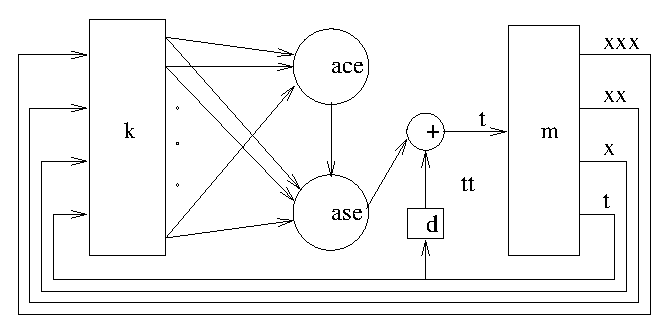
\includegraphics[width=0.9\columnwidth]{neural_network}
  \caption{Neural network architecture.}
  \label{fig:kase}
\end{figure}

The \emph{Simulated model} block reproduces the physics of the ball and plate
implementing the equations reported in Section~\ref{sec:sysmodel}.
According to its input, that is the updated plate angle, such a module
computes all the other system parameters which compose the system state $S$ as

$$S = [ \quad x \quad \dot{x} \quad \ddot{x} \quad \theta_x \quad ]^T.$$

The state $S$ is quantized through a \emph{Self Organizing Map} (SOM),
also known as \emph{Kohonen network}. 
The training parameters for such a network are reported in
Table~\ref{tab:kohonenparams}.
Note that a situation of $R_{min}$ equal to 1 implies that only the winning
neuron is updated.

\begin{table}
  \begin{center}
    \begin{tabular}{| l | c || r | }
      \hline
         $n$            & number of nodes                    & $700$ \\ \hline
         $n_r$          & number of rows                     & $35$  \\ \hline
         $n_c$          & number of columns                  & $20$  \\ \hline
         $\alpha_{max}$ & initial learning rate              & $0.4$ \\ \hline
         $\alpha_{min}$ & final learning rate                & $0.0$ \\ \hline
         $R_{max}$      & initial radius                     & $10$  \\ \hline
         $R_{min}$      & final radius                       & $1$   \\ \hline
         $T_{max}$      & max training duration (iterations) & $10^8$\\ \hline
    \end{tabular}
    \caption{Training parameters for the Kohonen network.}
    \label{tab:kohonenparams}
  \end{center}
\end{table}

The \emph{Associative Search Element} (ASE) associates a correct action in
response to a quantized input.
Moreover, the \emph{Adaptive Critic Element} (ACE) produces a secondary
reinforcement in order to let the ASE learn also when failures occur less
frequently.

The ASE's output consists of the plate angle variation, which is added to 
$\theta (t-\Delta t)$, to obtain the new plate angle.

The parameters of the \emph{Associative Search Element} (ASE) and
\emph{Adaptive Critic Element} (ACE) are reported respectively in
Table~\ref{tab:aseparams} and Table~\ref{tab:aceparams}. In order to
understand the meaning of such parameters, please refer to the handout
slides available at \cite{buttazzos_slides}.

\begin{table}
  \begin{center}
    \begin{tabular}{| l || r | }
      \hline
         $n$            & $700$ \\ \hline
         $\alpha$       & $10.0$ \\ \hline
         $\lambda$      & $0.75$ \\ \hline
    \end{tabular}
    \caption{ASE parameters.}
    \label{tab:aseparams}
  \end{center}
\end{table}

\begin{table}
  \begin{center}
    \begin{tabular}{| l || r | }
      \hline
         $n$            & $700$ \\ \hline
         $\lambda$      & $0.5$ \\ \hline
         $\beta$        & $0.4$ \\ \hline
         $\gamma$       & $1.0$ \\ \hline
    \end{tabular}
    \caption{ACE parameters.}
    \label{tab:aceparams}
  \end{center}
\end{table}

Initially, the failure condition was detected whenever the ball position hit
the plate borders.
Although this solution is simple and conceptually correct, unfortunately
it presents an unpleasant drawback, that is a slow and ineffective learning.
This effect is due to the fact that the simulations, in which the ball rolls 
from a border to another and back, are considered under control.
To avoid this kind of situation, the chosen approach consists in reducing
progressively the valid area during the simulation: at the beginning
such an area covers the whole plate; after a while, it shrinks proportionally
down to the lower bound. Each simulation not able to carry
the ball near the plate center in a limited time generates a failure.




\section{Results}
\label{sec:results}

The possible plate angles are bounded to be within the range
[-10$^\circ$, +10$^\circ$] with valid variations of $\pm$1$^\circ$:
such constraints are due to the fact that a wider range has a negative impact
on the ball acceleration, making the control more difficult. Moreover, varying
the plate angle beyond $\pm$1$^\circ$ implies an unrefined tuning and a
higher $\dot{\omega}$.

The control period for the simulation, $\Delta t$, is set to 20ms, being a
good trade-off between computational load and the system dynamics.
Longer intervals imply a harder learning because the ball shift widens
causing angle saturations and hence, a greater ball speed.

The plate is square and its side length is 0.40 meters.

The learning phase, reported in Figure~\ref{fig:learning}, took more than 30
hours executing about 27000 simulations.
Each simulation starts placing the ball in a random position on the plate,
initially horizontal, and executes at most $10^6$ learning steps.

\begin{figure}[htb]
  \centering
  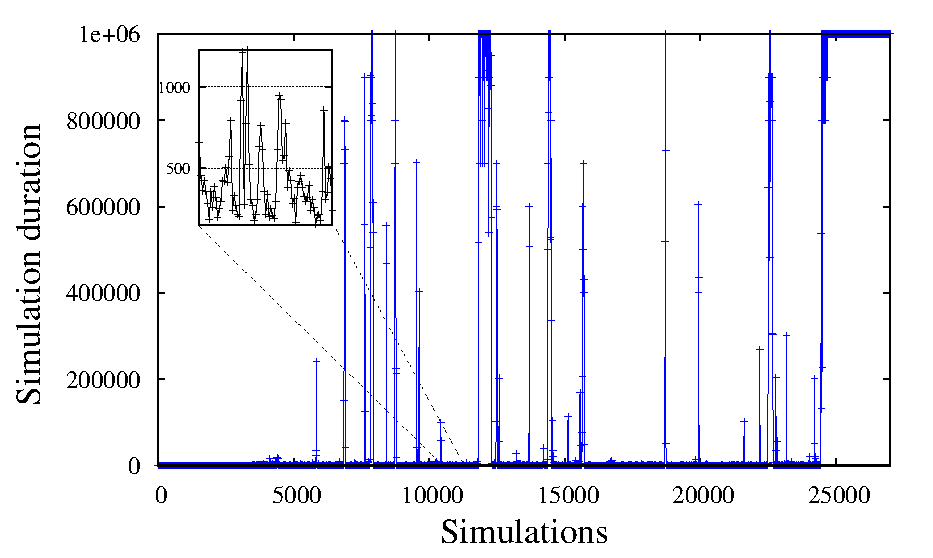
\includegraphics[width=0.9\columnwidth]{result.eps}
  \caption{Learning progress.}
  \label{fig:learning}
\end{figure}

Up to about 24000 simulations, failures occured few steps after the beginning
of the training procedure, except for some sporadic cases in which the ball was
well controlled.
From about 24000 simulations till the training session end (about 27000),
the networks were able to control the ball, keeping always it within the
red boundaries, until the simulation steps limit ($10^6$).

The networks always worked well during the next tests, being able to avoid
failures also when some moderate perturbations were applied through the
graphical program.

% end section




\section{Implementation}
\label{sec:impl}

The project is divided in two different programs written in C:
one for the neural network learning and the other for the graphical usage.
This approach helps to speed up the learning phase as the viewer executes a
learning update frequency equal to the Frames Per Second (FPS)
(more or less 30).
On the other hand, the dedicated program runs at the effective CPU speed,
executing more than thousands of steps per second.

The learning program is command-line and its synopsis is:
\begin{verbatim}
trainer [-k file] [-c file] [-s file] [-o file] [-r]
\end{verbatim}
where:
\begin{itemize}
    \item \emph{-k} specifies the file describing the Kohonen
             network that is deserialized and serialized at the beginning and
             at the end of the learning process, respectively.
             If the file does not exist or the option is not specified then the
             network is randomly initialized.
             Moreover, the neural network is not serialized if the option is
             not expressed;
    \item \emph{-c} is similar to \emph{-k} but concerns the ACE network;
    \item \emph{-s} is similar to \emph{-k} but concerns the ASE network;
    \item \emph{-o} writes in the specified file the learning advances in a
                    Comma Separated Values (CSV) format;
    \item \emph{-r} starts the learning. Without typing it, the program prints a
                    brief description in order to explain the option meanings
                    and exits.
\end{itemize}
The program execution is ended by sending it a SIGKILL signal (CTRL+C),
causing the neural networks serializations, if possible.

The visualization program uses the neural networks (only Kohonen and ASE)
to show the control usage.
Its synopsis is:
\begin{verbatim}
ball_and_plate [-k file] [-s file] [-r]
\end{verbatim}
where the options have the same meanings.

The graphical program, as shown in Figure~\ref{fig:screenshot}, presents a 
minimalistic layout reporting several basic information and a representation of
the ball and plate system, drawn using the OpenGL library.
The surface within the red boundaries represents the area
in which the controller has to keep the ball to avoid a failure.

\begin{figure}[htb]
  \centering
  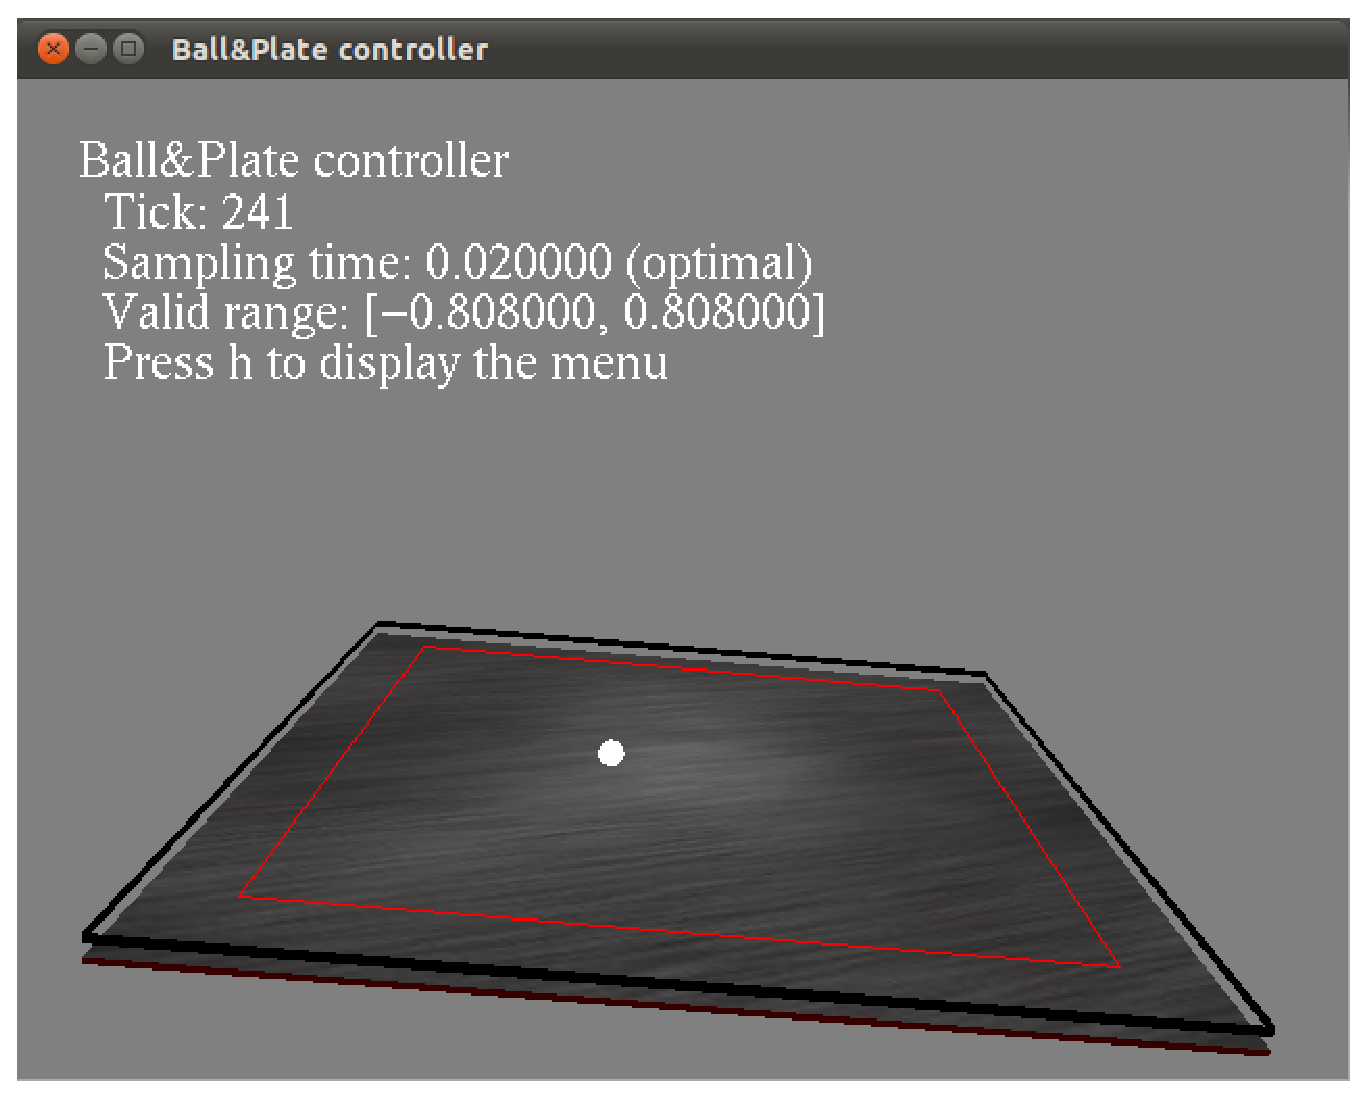
\includegraphics[width=0.9\columnwidth]{screenshot}
  \caption{Program screenshot.}
  \label{fig:screenshot}
\end{figure}

At the top, the program shows the tick number (how many control steps have been
executed), the sampling time (the time elapsed since the last control
event) and the side length of the red boudaries (as percentage of the whole
plate and according to the plate center).

Pressing either \emph{h} or \emph{H} key, the program displays a menu to
explain the available commands.
The keys \emph{w}, \emph{s}, \emph{a} and \emph{d} allow to rotate the 
point of view along the $X$ and $Z$ axis.
To perturbate the system, three features are available.
The \emph{b} key blocks the plate until another press of the same key.
The \emph{directional arrows} let the user to apply an external force to the
ball (not to the plate).
The last feature, enabled by the \emph{c} key, switches between the optimal and
real sampling: with the optimal approach the controller considers a
deterministic sampling every $\Delta t$ (the same used for the learning) while,
with real sampling, the controller works with the actual time elapsed since
the last screen refresh.
The last configuration depends on the graphical capability of the host machine
and the real sampling time usually lasts longer than the optimal one
causing a performance degradation so significant to make the controller
ineffective.
Finally, the \emph{p} and \emph{r} keys pause and reset the simulation,
respectively.

In order to simplify the programs invocations, two scripts are provided: 
\emph{trainer.sh} and \emph{ball\_and\_plate.sh}. Their task is to invoke the
relative programs passing them the pre-trained neural networks files.

% end section




\section{Conclusions}
\label{sec:conclusions}

This report presented a solution for the well-known Ball and Plate system
based on a neural controller.

%The physical model took into account almost all the forces, except for the
%rolling and sliding frictions.
Focusing on the controller, a Kohonen network encoded the system state to the
ASE, which computed the new plate angle. Moreover, the ACE produced a second
reinforcement for the ASE.

The results showed the convergence of the learning phase and the effectiveness
of the performed control.

%end section



\appendix

\section{How to use our tool}

This section briefly describes the procedure in order to run the trainer and
ball\_and\_plate programs both under UNIX and CYGWIN platforms.
In the following, for each platform, a list of the needed packages and console
commands is presented.

\subsection{GNU/Linux}

\textbf{Packages}

\begin{itemize}
\item freeglut3                                      
\item freeglut3-dev                                 
\end{itemize}

\noindent\textbf{Console commands}

\begin{verbatim}
$ cd Ball_and_Plate_controller
$ make 
$ ./trainer -k kohonen.nn -s ase.nn -c ace.nn -r
or
$ ./trainer.sh
$ ./ball_and_plate -k kohonen.nn -s ase.nn -r
or
$ ./ball_and_plate.sh
\end{verbatim}

\subsection{CYGWIN}

\textbf{Packages}

\begin{itemize}
\item gcc
\item make
\item opengl
\end{itemize}

\noindent\textbf{Console commands}

\begin{verbatim}
$ cd Ball_and_Plate_controller
$ make cygwin
$ ./trainer -k kohonen.nn -s ase.nn -c ace.nn -r
or
$ ./trainer.sh
$ ./ball_and_plate -k kohonen.nn -s ase.nn -r
or
$ ./ball_and_plate.sh
\end{verbatim}



\bibliographystyle{IEEEtran}
\bibliography{IEEEabrv,paper}

% that's all folks
\end{document}


